
\documentclass{article}\usepackage[]{graphicx}\usepackage[]{color}
% maxwidth is the original width if it is less than linewidth
% otherwise use linewidth (to make sure the graphics do not exceed the margin)
\makeatletter
\def\maxwidth{ %
  \ifdim\Gin@nat@width>\linewidth
    \linewidth
  \else
    \Gin@nat@width
  \fi
}
\makeatother

\definecolor{fgcolor}{rgb}{0.345, 0.345, 0.345}
\newcommand{\hlnum}[1]{\textcolor[rgb]{0.686,0.059,0.569}{#1}}%
\newcommand{\hlstr}[1]{\textcolor[rgb]{0.192,0.494,0.8}{#1}}%
\newcommand{\hlcom}[1]{\textcolor[rgb]{0.678,0.584,0.686}{\textit{#1}}}%
\newcommand{\hlopt}[1]{\textcolor[rgb]{0,0,0}{#1}}%
\newcommand{\hlstd}[1]{\textcolor[rgb]{0.345,0.345,0.345}{#1}}%
\newcommand{\hlkwa}[1]{\textcolor[rgb]{0.161,0.373,0.58}{\textbf{#1}}}%
\newcommand{\hlkwb}[1]{\textcolor[rgb]{0.69,0.353,0.396}{#1}}%
\newcommand{\hlkwc}[1]{\textcolor[rgb]{0.333,0.667,0.333}{#1}}%
\newcommand{\hlkwd}[1]{\textcolor[rgb]{0.737,0.353,0.396}{\textbf{#1}}}%
\let\hlipl\hlkwb

\usepackage{framed}
\makeatletter
\newenvironment{kframe}{%
 \def\at@end@of@kframe{}%
 \ifinner\ifhmode%
  \def\at@end@of@kframe{\end{minipage}}%
  \begin{minipage}{\columnwidth}%
 \fi\fi%
 \def\FrameCommand##1{\hskip\@totalleftmargin \hskip-\fboxsep
 \colorbox{shadecolor}{##1}\hskip-\fboxsep
     % There is no \\@totalrightmargin, so:
     \hskip-\linewidth \hskip-\@totalleftmargin \hskip\columnwidth}%
 \MakeFramed {\advance\hsize-\width
   \@totalleftmargin\z@ \linewidth\hsize
   \@setminipage}}%
 {\par\unskip\endMakeFramed%
 \at@end@of@kframe}
\makeatother

\definecolor{shadecolor}{rgb}{.97, .97, .97}
\definecolor{messagecolor}{rgb}{0, 0, 0}
\definecolor{warningcolor}{rgb}{1, 0, 1}
\definecolor{errorcolor}{rgb}{1, 0, 0}
\newenvironment{knitrout}{}{} % an empty environment to be redefined in TeX

\usepackage{alltt}
\usepackage{longtable}
\usepackage{geometry}
% \usepackage[round]{natbib}
\usepackage{natbib}
\bibliographystyle{abbrvnat}
\usepackage{graphicx}
\geometry{a4paper}
\usepackage[T1]{fontenc}
\usepackage[utf8]{inputenc}
\usepackage{authblk}
\usepackage[running]{lineno}
\usepackage{setspace}
\usepackage{courier}
% \usepackage{tabulary}
\usepackage{hyperref}
\doublespacing

\newcommand{\tom}[1]{{\textit{\color{red}{[#1]}}}}
\newcommand{\aldo}[1]{{\textit{\color{blue}{[#1]}}}}

\title{\texttt{popler}: an R package for extraction and synthesis of population time series from the long-term ecological research (LTER) network}
  \author[a,b,c]{Aldo Compagnoni\thanks{aldo.compagnoni@gmail.com}}
\author[a]{Andrew J. Bibian}
\author[a]{Brad M. Ochocki}
\author[b,c]{Sam Levin}
\author[d]{Kai Zhu}
\author[a]{Tom E.X. Miller}

\affil[a]{Department of BioSciences, Program in Ecology and Evolutionary Biology, Rice University, 6100 Main St, MS-170, Houston, TX 77005}
\affil[b]{Institute of Biology, Martin Luther University Halle-Wittenberg, Am Kirchtor 1, 06108 Halle (Saale), Germany}
\affil[c]{German Centre for Integrative Biodiversity Research (iDiv) Halle-Jena-Leipzig, Deutscher Platz 5e, 04103 Leipzig, Germany}
\affil[d]{Department of Environmental Studies, University of California, Santa Cruz, CA 95064, USA}

\renewcommand\Authands{ and }
\date{Running headline: The \texttt{popler} database and R package}
\IfFileExists{upquote.sty}{\usepackage{upquote}}{}
\begin{document}
% \SweaveOpts{concordance=TRUE}






\maketitle
% \tom{Tom's comments appear in red italics.}
% \aldo{Aldo's comments appear in blue italics.}

\newpage

\section*{Abstract}
%The Abstract must not exceed 350 words and should list the main results and conclusions, using simple, factual, numbered statements: Point 1: set the context for and purpose of the work; Point 2: indicate the approach and methods; Point 3: outline the main results; Point 4: identify the conclusions and the wider implications.



\begin{enumerate}

  \item Population dynamics play a central role in the historical and current development of fundamental and applied ecological science. The nascent culture of open data promises to increase the value of population dynamics studies to the field of ecology. However, synthesis of population data is constrained by the difficulty in identifying relevant datasets, by the heterogeneity of available data, and by access to raw (as opposed to aggregated or derived) observations.
  
  \item To obviate these issues, we built a relational database, \texttt{popler}, and its \texttt{R} client, library("popler"). \texttt{popler} accommodates the vast majority of population data under a common structure, and without the need for aggregating raw observations. library("popler") is  designed for users unfamiliar with the structure of the database and with the SQL language. This \texttt{R} library allows users to identify, download, explore, and cite datasets salient to their needs.
  
  \item We implemented popler as a PostgreSQL instance, where we stored population data originated by the United Stated Long Term Ecological Research (LTER) Network. Our focus on the US LTER data aims to leverage the untapped potential of this vast open data resource. The database currently contains 305 datasets from 25 LTER sites. \texttt{popler} is designed to accommodate automatic updates of existing datasets, and to accommodate additional datasets from LTER as well as non-LTER studies.
  
  \item The combination of the online database and the \texttt{R} library("popler") is a resource for data synthesis efforts in population ecology. The common structure of \texttt{popler} simplifies comparative analyses, and the availability of raw data confers flexibility in data analysis. library("popler") maximizes these opportunities by providing a user-friendly interface to the online database.

   \end{enumerate}
\section*{Keywords}
\linenumbers
open long-term population data, US Long Term Ecological Research Network data, online database, database structure, PostgreSQL, R package, comparative analysis


\newpage
\section*{Introduction}
% \linenumbers

Population dynamics – changes in species’ abundance and composition through time and space – are central to ecology for both applied and fundamental reasons. Populations are the building blocks of ecological dynamics at higher scales of organization, and examples abound showing how the study of population ecology improves understanding in evolution \citep{Metcalf2007}, community ecology \citep{Levine2009}, and ecosystem ecology \citep{Medvigy2009,Fisher2018}. Given their central role, studies of population dynamics will be an essential component in the advances allowed by the flourishing culture of open access and data synthesis.

The increase in freely available data is poised to change ecological science \citep{Laurance2016}. The rising focus on open data is clear in changing publishing standards, in the design of observational networks \citep{schimel2007neon}, and in the availability of previously proprietary data \citep{Kratz2003,Bechtold2005}. This deluge of open data holds promise to facilitate comparative analyses and to test the generality of ecological hypotheses. For population dynamics in particular, it is the increasing availability of long-term data that will likely yield the most substantial scientific advances, as long time series are required to detect trends in abundance \citep{Lindenmayer2012}, quantify temporal variance \citep{Compagnoni2016}, and identify endogenous \citep{Knape2012} or exogenous \citep{Hampton2013} drivers of population fluctuations.

There are currently three public databases that provide time series of population data. These are the Global Population Dynamics Database \citep[GPDD,][]{Inchausti2001}, the Living Planet Index \citep{loh2005living}, and BioTIME \citep{dornelas2018biotime}. These databases are an important resource for population biologists \citep[e.g.,][]{Knape2012}, but their characteristics make them optimal for a specific set of analyses. For example, the GPDD time series contain only one observation of population size or density per temporal replicate, BioTIME focuses on assemblage (i.e. multispecies) datasets, and the Living Planet Index contains information on single populations of conservation concern. These differences can be decisive in scientific inference. For example, LPI data indicate worldwide biodiversity declines, while BioTIME data indicate stable biodiversity due to higher species turnover. This is likely due to the focus of the LPI on species of conservation concern \citep{dornelas2019balance}. Finally, none of these three databases provides much data from experiments.

One of the best sources of publicly available long-term data is the Long-Term Ecological Research (LTER) network. The LTER was founded in 1980 and grew from the original six sites to, as of 2016, 28 sites throughout North America, Puerto Rico, French Polynesia, and Antarctica. Synthetic and comparative studies from the LTER network have made valuable contributions to ecological understanding \citep{Knapp2012}. However, the majority of LTER synthesis research has focused on ecological dynamics at the community (e.g. \cite{Wilcox2017}) and ecosystem (e.g. \cite{Knapp2001}) scales. Nevertheless, every LTER site collects population abundance data as one of its five core areas of continuous observations \citep{Callahan1984}. In our opinion these data, which have been accumulating since 1980, are under-used.

LTER population data provides two distinct advantages compared to existing databases. First, LTER data contains both single-species and assemblage datasets that might be free from the biases suggested for the LPI database. Assemblage datasets are expected to be an unbiased reflection of biodiversity trends \citep{dornelas2018biotime}, and LTER single-species studies are generally not focused on species of conservation concern. Second, many of the analyses on LTER experiments were published a few years after the start of manipulations. Hence, analysis of updated data from these LTER experiments could provide unique scientific insights.

One issue that may limit the use of LTER population data in synthetic, comparative studies is their heterogeneity. The structure of LTER data sets may be widely different, employing a variety of data types (counts of individuals, biomass estimates, percent cover, etc.), experimental designs driven by the priorities of particular PIs, and diverse replication schemes – idiosyncrasies that may be difficult to accommodate in a one-size-fits-all database. However, these challenges also present valuable opportunities. For example, the hierarchical replication structure of many LTER studies (e.g., subplots within plots within transects) can facilitate more sophisticated statistical investigation than would be possible with simpler, aggregated, or unreplicated data. %Ad-hoc software can greatly aid the discovery, querying, and comparison of datasets (e.g. \cite{Morris2013}). Dedicated software is therefore important to maximize the fruition, and the ultimate impact of publicly available datasets.

To overcome the issues posed by heterogeneous data structures, we developed \texttt{popler} (POPulation dynamics in Long-term Ecological Research), an online database of LTER population studies. This database defines a common data structure that can accommodate in principle all population data, and its SQL environment allows updates whenever new data becomes available. We also developed a companion R package to facilitate the identification, access, and manipulation of raw and heterogeneous population data. Our goals here are to provide introductions to the database and package. We focus on LTER time series, but expanding \texttt{popler} beyond the LTER network is a priority for future development.


\section*{The \texttt{popler} database}
To combine population data from the LTER network using a common structure, we identified a set of relevant variables (Table \ref{Tab:vars}) and organized them into a relational database. Here, we present the structure of the database in Fig. \ref{Fig:schema}, and we provide a simplified entity relationship diagram (ERD) in the supplementary material (Fig. \ref{Fig:simple_ERD}). In \texttt{popler} we stored ``raw'' data, meaning that we have not modified, edited, or aggregated the original observations.

For inclusion in \texttt{popler}, we only considered studies that included (1) repeated observations of populations or individuals through time, (2) at least five population censuses (as of database creation in 2017), and (3) taxonomic information associated with abundance observations (e.g., we excluded time series of functional groups). We provide technical details of database creation in Appendix S1.


The \texttt{popler} database currently contains data from 305 studies (122 of which are experimental) representing 4377 cumulative years of observations. On average, studies in \texttt{popler} contain 10.5 years of data (median: 7), with the longest study containing 67. The sampling designs are predominantly yearly (49\%) and sub-yearly (44\%), and only 6\% of designs sampled populations irregularly or less often than yearly. \texttt{popler} also contains abundant spatial replication, with studies containing a mean of 295 (median: 72) unique spatial replicates distributed across an average of 2.4 (median: 2) nested spatial replication levels. Finally, \texttt{popler} contains data from 665 plant species, 382 animal species, and 1 fungal species.


\subsection*{Population data}
We define ``population data'' as time-series of observations on the size or density of a population of a species or other taxonomic unit. Observations of population size are stored in a variable called \texttt{abundance\textunderscore observation} and can be measured as a count, biomass, density, or cover. These four types of population data are stored in the homonymous tables of the database (Fig. \ref{Fig:schema}A).

The population datasets contained in popler are always replicated temporally. Temporal replicates are identified with up to three variables: \texttt{year}, \texttt{month}, and \texttt{day}. Population data are also almost always spatially replicated, and spatial replicates are often nested, where for example a study might include separate sites, each of which contains intermediate spatial replicates (e.g. a transect, a block), which in turn contain the smallest spatial replicate at which observations are made (e.g. a plot, a quadrat). The hypothetical study described above would have three nested levels of spatial replication, identified by three numbered \texttt{spatial\textunderscore replication} variables. In \texttt{popler}, we accommodate data sets with up to five spatial replication levels (Table \ref{Tab:vars}). We call the first and therefore largest spatial replicate ``study site'' (Fig. \ref{Fig:schema}C). Note that this does not refer to the LTER site, one of the 28 NSF-supported locations (Table \ref{Tab:S3}).

\texttt{popler} contains both observational and experimental studies. Experimental datasets contain information on one or more experimental treatments. Popler accommodates information on up to three experimental treatments, identified by three numbered \texttt{treatment\textunderscore type} variables (Table \ref{Tab:vars}). 

Most datasets also contain one or more variables in addition to the ones described above which we store in a character variable called \texttt{covariates} (Table \ref{Tab:vars}). These are variables that do not conform to our data model. \texttt{covariates} stores in each row, the content an arbitrary number of such non-conforming variables. \texttt{covariates} can be useful, for example, for time series that contain information on population structure. In these datasets, observations on population size are grouped based on subdivisions of the entire population, such as males and females, large and small individuals, etc. We identify these datasets through a variable in the metadata \texttt{structured\textunderscore data} (Table \ref{Tab:S2}).

Finally, in addition to time series of abundance, \texttt{popler} contains individual-level data. This data provides information on the attributes of the individuals, or a subset thereof, that make up a population. We store this information in a dedicated table (''Individual'', Fig. \ref{Fig:schema}A). As individual attributes we consider variables that describe identity, size, sex, life stage or status (e.g. reproductive or non-reproductive). We refer to these individual attributes with the term ``structure'': \texttt{popler} accommodates data sets that measure up to four types of structure simultaneously. We store these data in up to four numbered \texttt{structure\textunderscore type} variables. While these data are not population time series; we chose to include them in \texttt{popler} because they provide information on demographic transitions that can be used to derive estimates of population growth. Moreover, in the cases of datasets that sample all of the individuals in a population, individuals can be aggregated (i.e. summed) as a measure of population size.


\subsection*{Taxonomic information}
Each observation corresponds to a taxonomic unit (Fig. \ref{Fig:schema}B), typically a species or a genus, but also include data that refer to a higher taxonomic rank, such as family, or order. %The majority of data sets provided by the LTER include multiple taxa, so each observation regarding population size or individual attribute is associated with a unique taxonomic unit.--seems redundant
\texttt{popler} provides 15 taxonomic ranks, and two additional variables that refer to how taxonomic information is recorded in the original datasets. The additional variables are \texttt{sppcode}, which are taxon-specific alphanumeric codes, and \texttt{common\textunderscore name}, the common name of each taxonomic unit (Table S1). \texttt{popler} also allows to store accepted taxonomic information in an additional table (Fig. \ref{Fig:schema}B). This table accounts for ambiguities contained in the raw taxonomic data, which originate by the dynamic changes in species classifications \citep{Chamberlain2013}. Further versions of popler will populate this second table with the accepted taxonomic units (which include  taxonomic information above the level of genus) provided by the R package \texttt{taxize} \citep{Chamberlain2013}.

\subsection*{Study site}
We stored the locations of datasets by recording the latitude (\texttt{lat\textunderscore study\textunderscore site}) and longitude (\texttt{lng\textunderscore study\textunderscore site}) of study sites (Fig. \ref{Fig:schema}C). Storing this information in a separate table allows for explicit connections between independent data sets collected at the same locations within LTER sites. 

\subsection*{Metadata}
The metadata table (Table \ref{Tab:S2}) provides information on temporal and spatial replication, and study design (Fig. \ref{Fig:schema}D), including title, link to online metadata, contact information for data originators, and the type of data provided by the dataset (i.e., which of the five tables in Fig. \ref{Fig:schema}A the data is stored in). All remaining metadata is related to the variables stored in the tables of \ref{Fig:schema}A and \ref{Fig:schema}B. First, some population datasets subdivide the population in groups that share the same characteristic (e.g. sex, developmental stage, age). These datasets, however, are not individual data (Fig. \ref{Fig:schema}D). We flag these datasets through the variable \texttt{structured\textunderscore data}. Second, we provide the years elapsed between the first and last observation (\texttt{duration\textunderscore years}), and the sampling frequency (\texttt{samplefreq}). Third, we provide the number of levels of nested spatial replicates, and the number of replicates for each spatially nested level. Fourth, we show whether studies focus on a single species or on multiple species through the \texttt{community} variable. Fifth, we identify studies as observational or experimental (\texttt{studytype}). If a study is experimental, we provide information on the type of treatments imposed by the study (\texttt{treatment\textunderscore type\textunderscore n}) and, when available, which one is the control treatment (\texttt{control\textunderscore group}). Finally, we report information on the data stored in the \texttt{abundance\textunderscore observation} variable: its units of measure (\texttt{samplingunits}), the area over which this abundance data was observed\\ (\texttt{spatial\textunderscore replication\textunderscore level\textunderscore n\textunderscore extent} and\\ \texttt{spatial\textunderscore replication\textunderscore level\textunderscore n\textunderscore extent\textunderscore units}), and in case the data was aggregated across space or time we flag these data as derived (\texttt{derived}).

\section*{The \texttt{popler} package}
The \texttt{popler} \texttt{R} package consists of three core functions that allow users to browse and retrieve data from the database (Fig. \ref{Fig:pack_funs}). In order of intended use, these functions are: \texttt{pplr\textunderscore dictionary()}, \texttt{pplr\textunderscore browse()}, and \texttt{pplr\textunderscore getdata()}.

\subsection*{The \texttt{pplr\textunderscore dictionary()} function}
The dictionary function is a good place for new users to begin working with \texttt{popler} (Fig. \ref{Fig:pack_funs}). With no arguments provided, this function returns a subset of the most useful metadata variables associated with each  dataset (Fig. \ref{Fig:schema}). Providing argument \texttt{full\textunderscore tbl = TRUE} returns all 77 metadata variables. Each one of these variable names can be provided as an argument to \texttt{pplr\textunderscore dictionary()}, which then returns the possible unique values of the variable. For example, \texttt{pplr\textunderscore dictionary(lterid)} returns the three letter codes of the LTER network sites included in \texttt{popler}. For numeric variables such as \texttt{duration\textunderscore years}, \texttt{pplr\textunderscore dictionary()} returns a summary including quantiles, mean, and median. 

\subsection*{The \texttt{pplr\textunderscore browse()} function}
Once the user is familiar with the meaning and content of the variables that define \texttt{popler} datasets, they are ready to dig deeper using \texttt{pplr\textunderscore browse()} (Fig. \ref{Fig:pack_funs}). Running \texttt{pplr\textunderscore browse()} without arguments provides the metadata from the entire contents of the database. This will be a $305 by 20$ data frame, with each row corresponding to a study and each column corresponding to a variable defined by \texttt{pplr\textunderscore dictionary()}.

The full strength of \texttt{pplr\textunderscore browse()} is achieved by subsetting studies according to desired criteria using logical expressions. For example, the user might want to consider only studies whose duration is 30 years or greater, which can be subsetted with:
\begin{knitrout}
\definecolor{shadecolor}{rgb}{0.969, 0.969, 0.969}\color{fgcolor}\begin{kframe}
\begin{alltt}
\hlstd{LTER_30} \hlkwb{<-} \hlkwd{pplr_browse}\hlstd{( duration_years} \hlopt{>} \hlnum{29}\hlstd{)}
\end{alltt}
\end{kframe}
\end{knitrout}
This operation will create the object \texttt{LTER\textunderscore 30}, which provides metadata for the data sets that satisfy the specified criterion. Multiple criteria may be combined. For example, 30+ year studies of plants can be browsed with
\begin{knitrout}
\definecolor{shadecolor}{rgb}{0.969, 0.969, 0.969}\color{fgcolor}\begin{kframe}
\begin{alltt}
\hlstd{LTER_30_plants} \hlkwb{<-} \hlkwd{pplr_browse}\hlstd{( duration_years} \hlopt{>} \hlnum{29} \hlopt{&}
                               \hlstd{kingdom} \hlopt{==} \hlstr{"Plantae"}\hlstd{)}
\end{alltt}
\end{kframe}
\end{knitrout}
To facilitate data exploration, \texttt{pplr\textunderscore browse()} output can be printed in a more readable settings by providing \texttt{report = TRUE} as an argument, which opens up a formatted html document. The metadata provided by \texttt{pplr\textunderscore browse()} not only contains information on the characteristics of a study but also information on how to cite the study, its unique identifiers, including digital object identifier (DOI), and the contact information of study PIs. 


\subsection*{The \texttt{pplr\textunderscore get\textunderscore data()} function}

Once data sets of interest have been identified, \texttt{pplr\textunderscore get\textunderscore data()} downloads the data from a server that hosts the database. This function can take as its first argument a \texttt{browse} object, a logical expression, or both. The data downloaded from \texttt{popler} are in ``long'' form, meaning that each row of data reports a single measure of population size, and separate variables indicate the temporal and spatial replicate, taxa, etc. This format makes it easy to further subset downloaded datasets with the aim of visualization and analysis. 

\subsection*{Ancillary functions}
\texttt{popler} also provides three additional functions to open the url of the original dataset, unpack covariates, and provide a citation for each dataset. First, the function \texttt{metadata\textunderscore url()} launches the online study description in a web browser. Second, the \texttt{cov\textunderscore unpack()} function transforms the \texttt{covariates} variable into a data frame (which \texttt{pplr\textunderscore get\textunderscore data()} does not provide by default). Third, \texttt{pplr\textunderscore citation()} generates a citation for the originators or each data set. 

\section*{Limitations and opportunities for development}
Working with raw, spatially replicated, and non-aggregated data provides key advantages in quantitative analyses of population dynamics which were a driving force behind the development of \texttt{popler}. However, users need to examine individual datasets and the associated online study descriptions to understand their peculiarities. Single datasets have unique idiosyncrasies that require vetting. For example, many datasets have gaps or changes in the sampling design during the length of the study, or the  \texttt{covariates} variable can hold key information. Hence, we urge authors to consult the online documentation of the original datasets.

In the future, there are opportunities to increase the size of \texttt{popler} and expand its scope. First, because many of the studies included in \texttt{popler} are ongoing, there will be opportunities to run regular updates aimed at including new observations in \texttt{popler}. Second, because our schema (Fig. \ref{Fig:schema}) is very general, the database could be expanded to include population datasets outside of the LTER network. Third, it would be valuable to explicitly associate \texttt{popler}'s population-level data with environmental drivers, especially climate. Thus, it is our intention and hope that the resources provided by \texttt{popler} will advance ecological understanding of population dynamics within the LTER network, and more generally.

\section*{Acknowledgements}
We thank Trevor Drees and Michael Saucedo for assistance in database development, Maurizio Compagnoni for assistance in database management, and Scott Chamberlain for developing the API to query the online database. Support for database and package development was provided by the US National Science Foundation to TEXM (DEB-1543651). This research was additionally supported by a Julian Huxley Faculty Fellowship from Rice University and a Faculty Research Grant awarded by the Committee on Research from the University of California, Santa Cruz (KZ). The LTER network is supported by the US National Science Foundation.

\section*{Authors' contributions}
AC, AB, KZ, MO, TEXM designed and built the database. AC AB, KZ, BD, SM, and TEXM designed and built the R package. AC and TEXM led the writing of the manuscript. All authors contributed to manuscript drafts and gave final approval for publication.

\section*{Data Availability}
The \texttt{popler} R package is publicly available at https://github.com/ropensci/popler.

\newpage
\bibliography{popler}

\newpage
 \begin{table}[h!]
%\begin{longtable}{p{10cm} p{5cm}}
  \caption{Variables used to store population or individual data in \texttt{popler}.}
  \label{Tab:vars}

  % \caption{Variables used to store population or individual data in \texttt{popler}.}
  % \label{Tab:vars}
   \begin{center}
     \begin{tabular}{l p{8cm}}
      \hline
      Variable & Description \\
      \hline
      \texttt{abundance\textunderscore observation} & {Measure of population abundance at a specific time and location. This variable measures abundance as a count, biomass, density, or cover. For individual data sets this variable is always equal to 1, because each attribute or set of attributes refer to a single individual.} \\
      \texttt{day} & Day of observation\\
      \texttt{month} & Month of observation\\
      \texttt{year} & Year of observation\\
      \texttt{spatial\textunderscore replicate\textunderscore n} & {The $n^{th}$ level of spatial replication, where \texttt{spatial\textunderscore replicate\textunderscore 1} is the study site. \texttt{popler} accommodates up to five levels of spatial replication.}\\
      \texttt{treatment\textunderscore type\textunderscore n} & {For datasets originating from an experimental study, the $n^{th}$ treatment. \texttt{popler} popler accommodates up to three treatments.}\\
      \texttt{covariates} & Ancillary observations that do not fall into the standard schema of \texttt{popler}.\\
      \texttt{structure\textunderscore type\textunderscore n} & {For individual data, these variables measure the $n^{th}$ attribute of individuals (identity, size, sex, status, stage). \texttt{popler} accommodates up to four structure types per dataset.}\\
      \hline
     \end{tabular}
   \end{center}
 \end{table}
%\end{longtable}

\newpage
\begin{figure}[h!]
  \begin{center}
    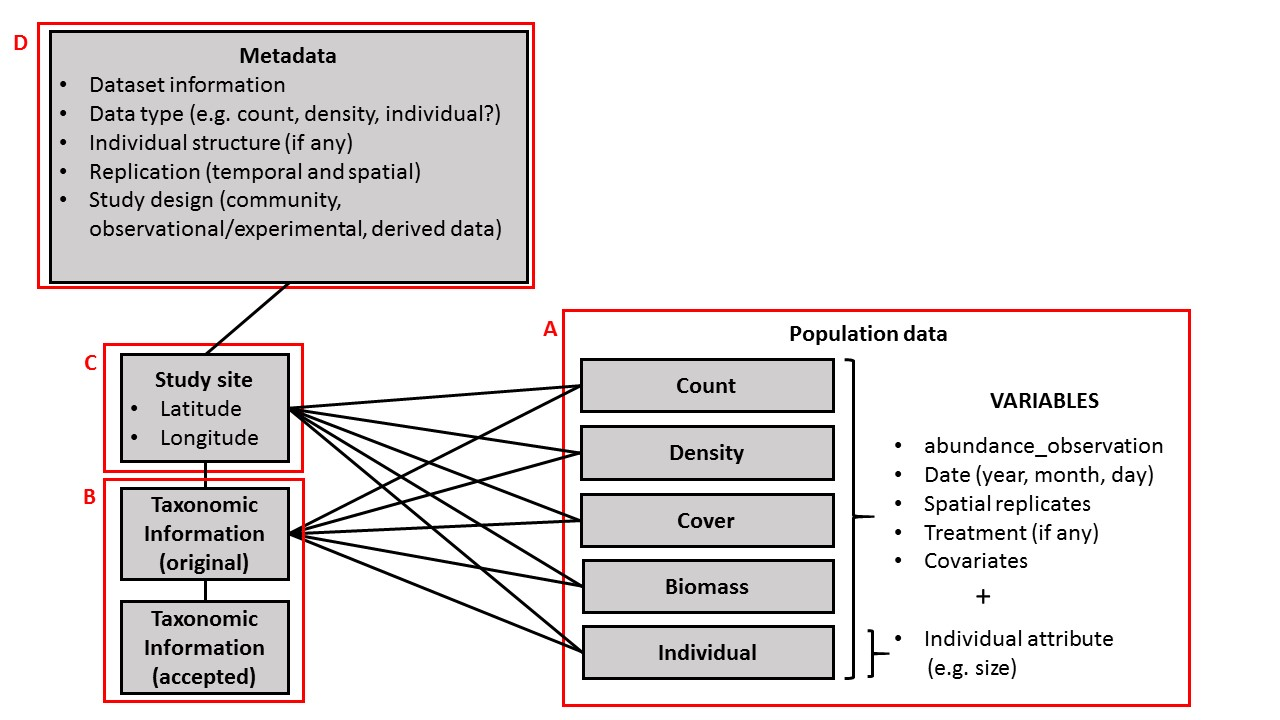
\includegraphics[scale=0.4]{schema}
    \caption{Schematic representation of the entity relationship diagram of the \texttt{popler} database. \texttt{popler} provides metadata on the studies that originated abundance data points (D). This metadata contains information on the unique identifiers of each study, on its design (observational or experimental), temporal and spatial replication. \texttt{popler} stores the latitude and longitude of the study site (C). Each abundance data point corresponds to a specific taxonomic unit (B). Finally, the time series of population data collected in a study can be of four different types (count, density, biomass, cover), or they may be individual data with attributes such as size or sex (A).}
    \label{Fig:schema}
  \end{center}
\end{figure}


\newpage
\begin{figure}[h!]
  \begin{center}
    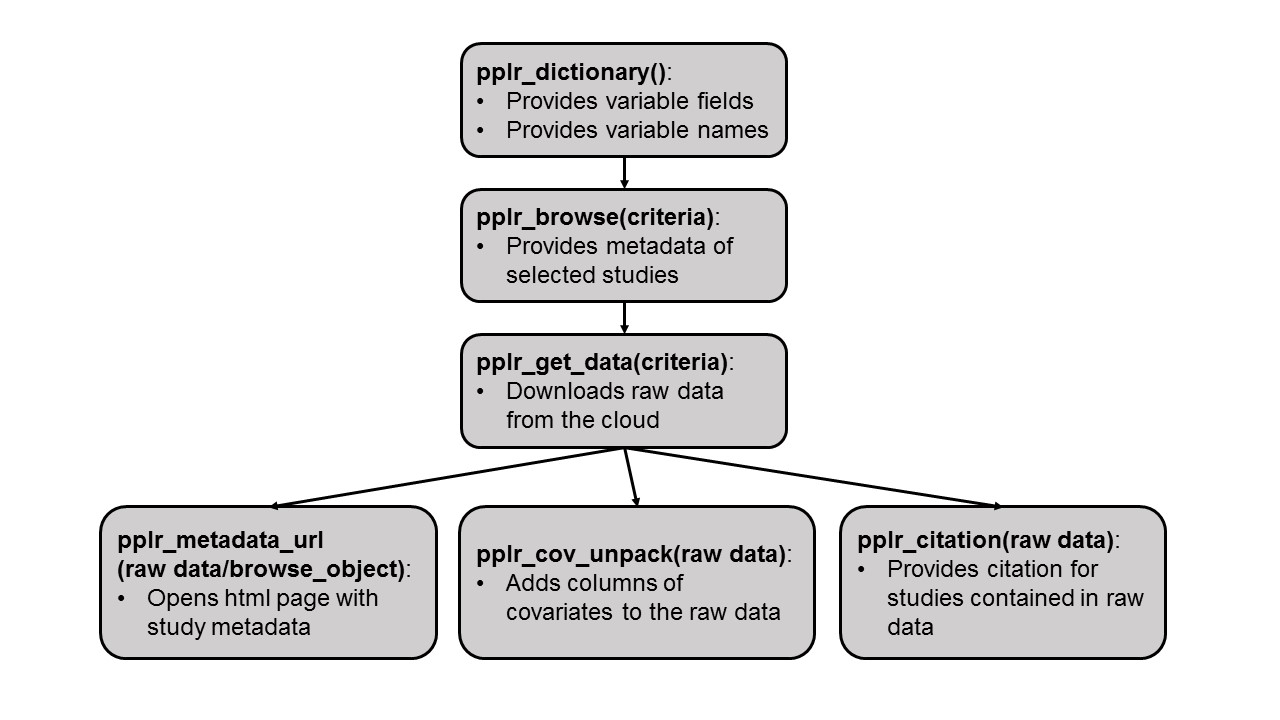
\includegraphics[scale=0.4]{pack_funs}
    \caption{Suggested workflow when using the \texttt{popler} R package to interface with the homonymous online database. The function \texttt{pplr\textunderscore dictionary()} refers to the variables of the metadata that describe the data sets contained in \texttt{popler}. \texttt{pplr\textunderscore dictionary()} describes these variables and returns their possible values. This information advises which criteria to use when subsetting \texttt{popler}. The user can provide a criterion (that is, a logical statement) to browse the metadata, using \texttt{pplr\textunderscore browse()}, or to download data using \texttt{pplr\textunderscore get\textunderscore data()}. Moreover, the output of \texttt{pplr\textunderscore get\textunderscore data()} (a data frame) can be the argument of three ancillary functions: \texttt{pplr\textunderscore metadata\textunderscore url()} opens the webpage containing the original dataset and their associated online metadata. \texttt{pplr\textunderscore cov\textunderscore unpack()} can be used to format the covariates contained in a raw data object into separate columns of a data frame. Finally, \texttt{pplr\textunderscore citation()} provides a citation for the downloaded data set(s).}
    \label{Fig:pack_funs}
  \end{center}
\end{figure}

%\newpage
%\begin{figure}[h!]
%  \begin{center}
%    \includegraphics[scale=0.8]{reportT}
%    \caption{The html output of function \texttt{pplr\textunderscore browse()} when argument \texttt{report = TRUE} is supplied.}
%    \label{Fig:reportT}
%  \end{center}
%\end{figure}

%\newpage
%\begin{figure}[h!]
%  \begin{center}
%    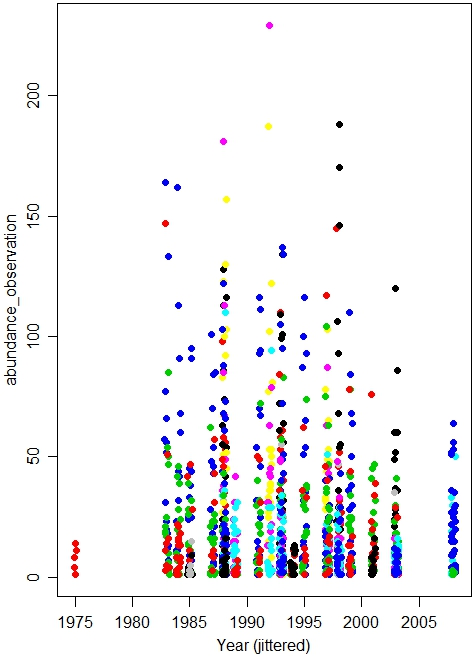
\includegraphics[scale=0.8]{BNZ_plot}
%    \caption{Time series of \textit{Viburnum edule} abundance counts at Bonanza Creek LTER. Dots show the number of individuals observed at each study site (y-axis) in each year (x-axis). Each color corresponds to a study site, the largest scale of spatial replication in \texttt{popler}. However, in this study each site contains 20 plots, a nested spatial replicate. Therefore, this plot shows multiple points per site each year.}
%    \label{Fig:BNZ_plot}
%  \end{center}
%\end{figure}

%\newpage
%\begin{figure}[h!]
%  \begin{center}
%    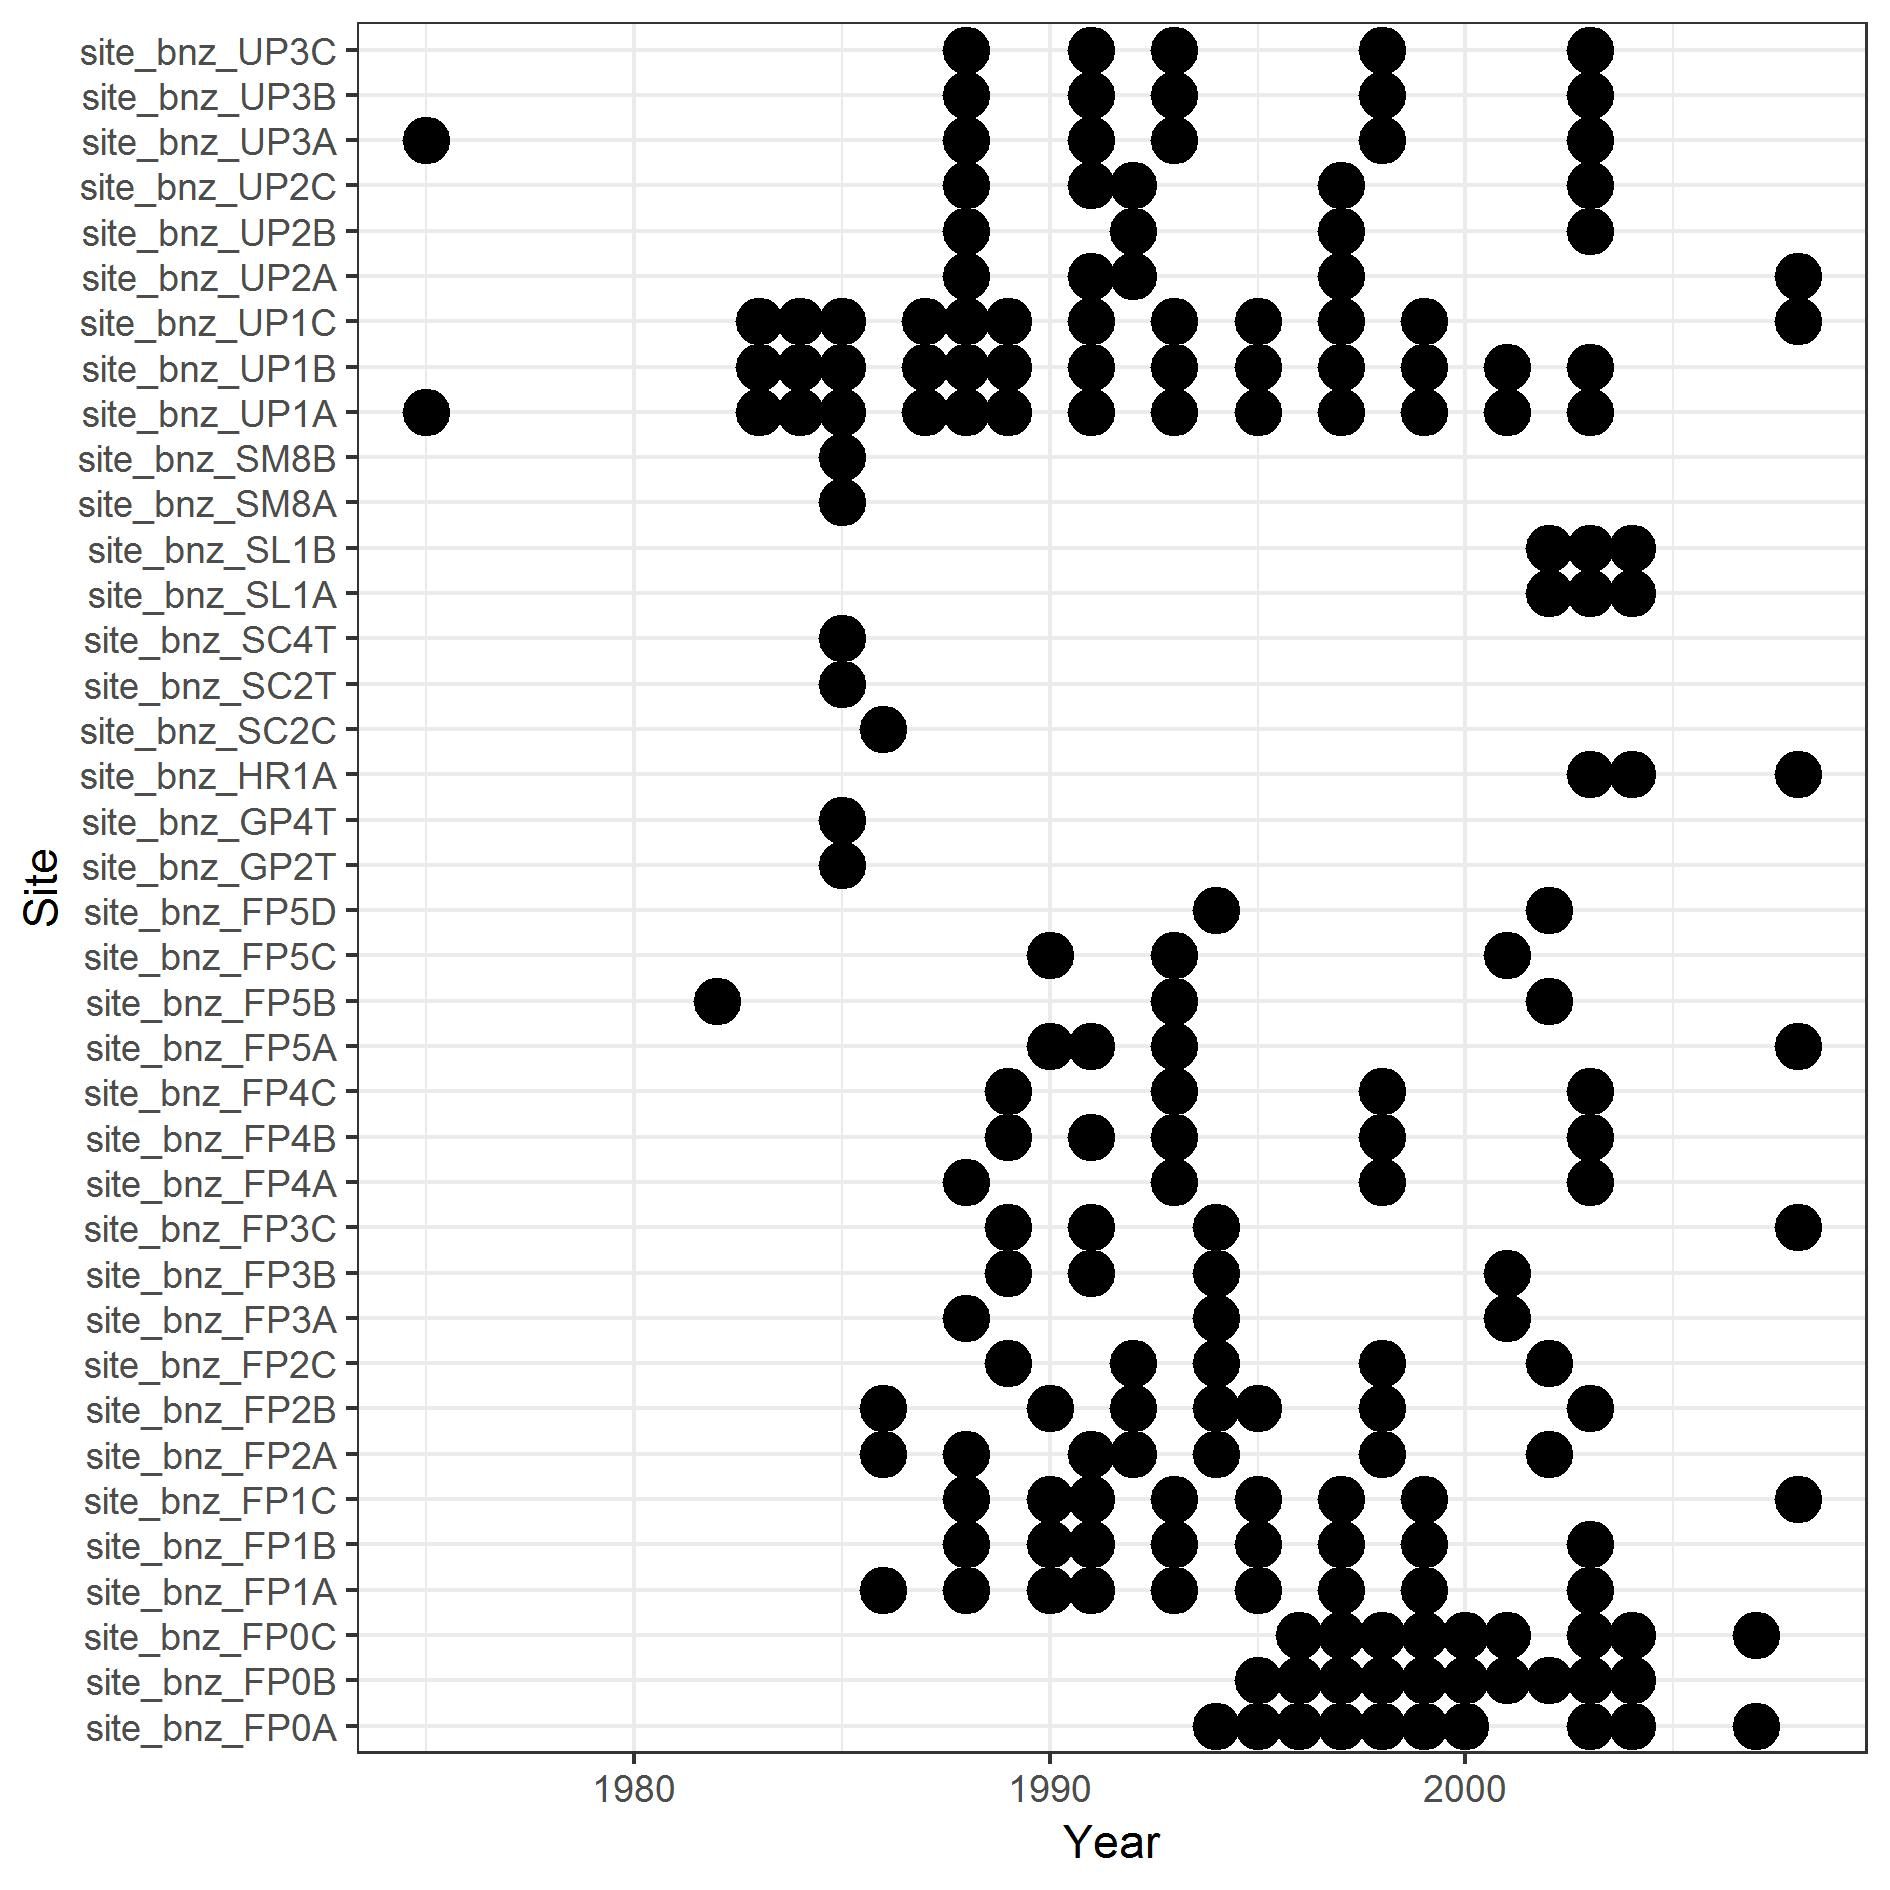
\includegraphics[scale=0.8]{BNZ_rep}
%    \caption{The degree of heterogeneity in the spatio-temporal sampling of the Bonanza Creek dataset. Dots show when count data is available at a particular site (y-axis) and at a particular year (x-axis). In this plot, count data refers to the whole plant community, rather than a single species.}
%    \label{Fig:BNZ_rep}
%  \end{center}
%\end{figure}


\newpage

\section*{Appendix S1: Pre-processing \texttt{popler} data}
Before uploading datasets into the online \texttt{popler} database, we combined datasets, transformed datasets from wide to long form, converted non-ASCII characters, and modified ambiguous study site names.

The variables of many datasets were contained in two or more separate files, which we combined in a single file. When the original dataset provided data in wide form, we transformed it into long form. In wide form datasets, abundance data associated with different species was stored in separate columns. \texttt{popler} stores these datasets in long form, whereby each row of abundance data is related to a specific taxonomic unit in the table containing taxonomic information (Fig. \ref{Fig:schema}B). We converted all data in ASCII format, because the encoding of the database is the UTF-8. We often re-defined study site names to unambiguously associate them with one of the 26 LTER sites. Many site names are alphanumeric codes (e.g. ``U1'') which can overlap across several LTER sites. Hence, we changed site names following a standard formula (namely, from ``U1'' to ``site\textunderscore sbc\textunderscore U1'', where ``sbc'' refers to the Santa Barbara coastal LTER site).

In a handful of cases, we removed single data rows from the original dataset. These data rows were associated with two types of typos in the original dataset. First, some abundance observations were not associated with a time of observation. We removed this data because \texttt{popler} can only accommodate population information associated with a time of observation. Second, a handful of abundance data points were clear typos (e.g. the letter ``l'' instead of a numeric value). We substituted these data points with a missing value. We uploaded these pre-processed datasets in the \texttt{popler} database through a Graphic User Interface developed in Python using libraries panda and pyqt5.

\newpage
\setcounter{table}{0}
\renewcommand{\thetable}{S\arabic{table}}

 \begin{table}[h!]
%\begin{longtable}{p{10cm} p{5cm}}
  \caption{Taxonomic variables contained in the popler table on original taxonomic information.}
  \label{Tab:S1}
   \begin{center}
     \begin{tabular}{l}
      \hline
      Variable\\
      \hline
      \texttt{sppcode} \\
      \texttt{kingdom}\\
      \texttt{subkingdom}\\
      \texttt{infrakingdom}\\
      \texttt{superdivision}\\
      \texttt{division}\\
      \texttt{subdivision}\\
      \texttt{superphylum}\\
      \texttt{phylum}\\
      \texttt{subphylum}\\
      \texttt{class}\\
      \texttt{subclass}\\
      \texttt{order}\\
      \texttt{family}\\
      \texttt{genus}\\
      \texttt{species}\\
      \texttt{common\textunderscore name}\\
      \hline
     \end{tabular}
   \end{center}
 \end{table}
%\end{longtable}

\newpage
 %\begin{table}[h!]
   %\caption{Metadata variables used to describe the datasets stored in \texttt{popler.}}
   %\label{Tab:S2}
   %\begin{center}
   %\begin{tabular}{p{10cm} p{5cm}}
    \begin{longtable}{p{10cm} p{5cm}}
      \caption{Metadata variables used to describe the datasets stored in \texttt{popler.}}
      \label{Tab:S2}\\
      \hline
      Variable & Description \\
      \hline
\texttt{proj\textunderscore metadat\textunderscore key} & {Unique ID} \\
\texttt{lter\textunderscore project\textunderscore key} & {ID of LTER site} \\
\texttt{lter\textunderscore project\textunderscore key} & {ID of LTER site} \\
\texttt{title} & {Title of study} \\
\texttt{samplingunits} & {Unit of measure (if any) referred to population data.} \\
\texttt{datatype} & {Data type: count, biomass, cover, density, and individual. These correspond to the tables in Fig. 1A.} \\
\texttt{structured\textunderscore data} & {If data type is not individual, but the abundance observations refer to sub-groups of the population based on, for example, sex, developmental stage, or age)} \\
\texttt{structured\textunderscore type\textunderscore n} & {If individual data, this shows what type of structure is stored. A study can contain up to $n = 4$ types of structure.}\\
\texttt{structured\textunderscore type\textunderscore n\textunderscore units} & {Unit of measure (if any) referred to structure data.}\\
\texttt{studystartyr} & {Start year of the study} \\
\texttt{studyendyr} & {End year of the study} \\
\texttt{duration\textunderscore years} & {Duration of the study in years} \\
\texttt{samplefreq} & {Frequency of population census} \\
\texttt{studytype} & {Whether study is observational or experimental} \\
\texttt{community} & {Whether study includes single taxon (\texttt{community = F}) or multiple taxa (\texttt{community = T})} \\
\texttt{spatial\textunderscore replication\textunderscore level\textunderscore n\textunderscore extent} & {Extent of spatial replication level number $n$. A dataset can have up to to 5 replication levels.} \\
\texttt{spatial\textunderscore replication\textunderscore level\textunderscore n\textunderscore extent\textunderscore units} & {Unit of spatial extent of the $n$ spatial replication level.} \\
\texttt{spatial\textunderscore replication\textunderscore level\textunderscore n\textunderscore label} & {Label of the spatial replication level (e.g. transect, plot, quadrat, ect.). The label of spatial replication level 1 is ``site''.} \\
\texttt{spatial\textunderscore replication\textunderscore level\textunderscore n\textunderscore number\textunderscore of\textunderscore unique\textunderscore reps} & {The number of unique replicates for the $n$th level of spatial replication.} \\
\texttt{treatment\textunderscore type\textunderscore n} & {The type of treatment (e.g. resource manipulation). A study can contain up to \texttt{n = 3} treatments.} \\
\texttt{control\textunderscore group} & {If study is experimental, this shows the field(s) that identify the control replicate.} \\
\texttt{derived} & {Is population size data raw, or is it derived (e.g. it is aggregated)?} \\
\texttt{authors} & {Author(s) of the original dataset} \\
\texttt{authors\textunderscore contact} & {Email address(es) of the author(s) associated with the original dataset.} \\
\texttt{metalink} & {url of the original dataset} \\
\texttt{knbid} & {Knowledge Network for Biocomplexity identifier.} \\
      \hline
    \end{longtable}
    %\end{tabular}
   %\end{center}
 %\end{table}     
     
\newpage     
 \begin{table}[h!]
%\begin{longtable}{p{10cm} p{5cm}}
  \caption{LTER identification acronyms and their meaning as used in the \texttt{popler} database.}
  \label{Tab:S3}
   \begin{center}
     \begin{tabular}{l l}
      \hline
      Variable & LTER name\\
      \hline
AND & Andrew Forest LTER \\                        
ARC & Arctic LTER \\                               
BES & Baltimore Ecosystem Study \\                 
BNZ & Bonanza Creek LTER \\                        
CAP & Central Arizona - Phoneix LTER \\            
CCE & California Current Ecosystem LTER \\         
CDR & Cedar Creek Ecosystem Science Reserve LTER \\
CWT & Coweeta LTER \\                              
FCE & Florida Coastal Everglades LTER \\           
GCE & Georgia Coastal Ecosystems LTER \\           
HBR & Hubbard Brook LTER \\                        
HFR & Harvard Forest LTER \\                       
JRN & Jornada Basin LTER \\                        
KBS & Kellogg Biological Station LTER \\           
KNZ & Konza Prairie LTER \\                        
LNO & LTER Network Office \\                       
LUQ & Luquillo LTER \\                             
MCM & McMurdo Dry Valleys LTER \\                  
MCR & Moorea Coral Reef LTER \\                    
NCO & LTER Network Communications Office \\        
NTL & North Temperate Lakes LTER \\                
NWT & Niwot Ridge LTER \\                          
PAL & Palmer Antarctica LTER \\                    
PIE & Plum Island Ecosystems LTER \\               
SBC & Santa Barbara Coastal LTER \\                
SEV & Sevilleta LTER  \\                           
SGS & Shortgrass Steppe LTER \\                    
VCR & Virginia Coastal Reserve LTER \\
      \hline
     \end{tabular}
   \end{center}
 \end{table}
%\end{longtable}

\setcounter{figure}{0}
\renewcommand{\thefigure}{S\arabic{figure}}

\newpage
\begin{figure}[h!]
  \begin{center}
    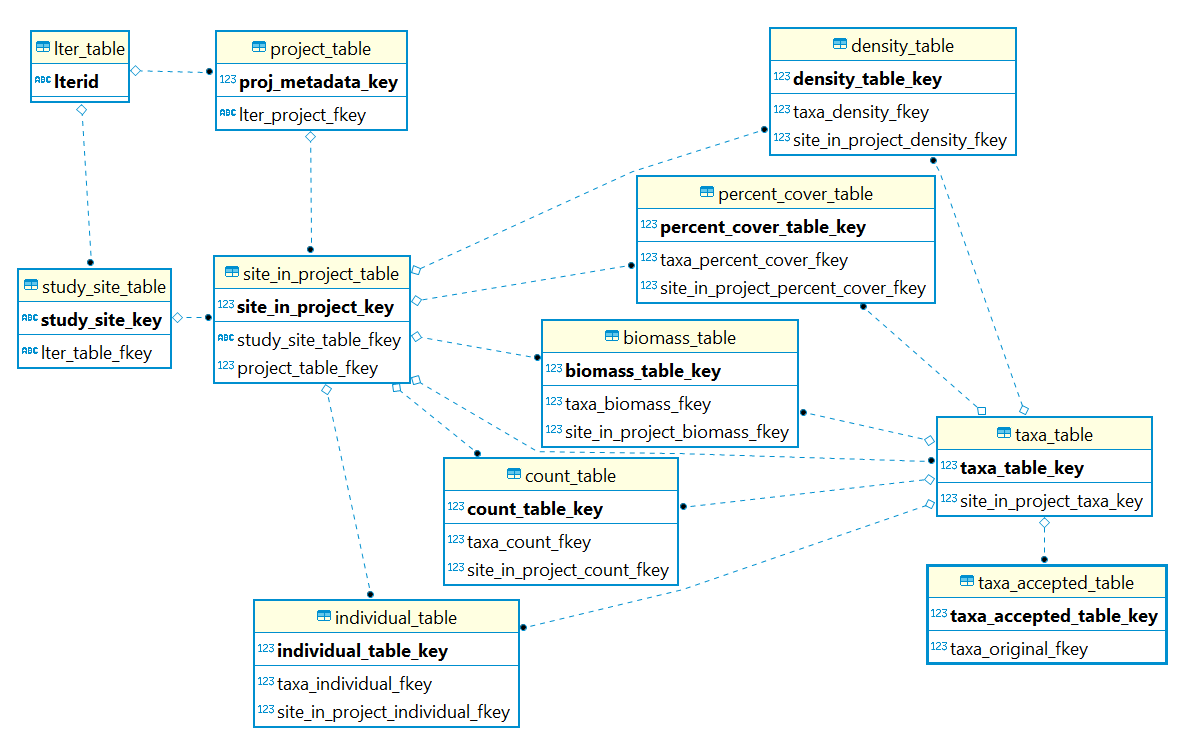
\includegraphics[scale=0.4]{simple_ERD}
    \caption{Simplified entity relationship diagram of the \texttt{popler} database. This figure shows table names, primary keys, and foreign keys of the \texttt{popler} database. It does not show, however, the other variable names contained in each table.}
    \label{Fig:simple_ERD}
  \end{center}
\end{figure}


\end{document}
